
\definecolor{ccccccc}{RGB}{204,204,204}
\definecolor{cff8080}{RGB}{255,128,128}


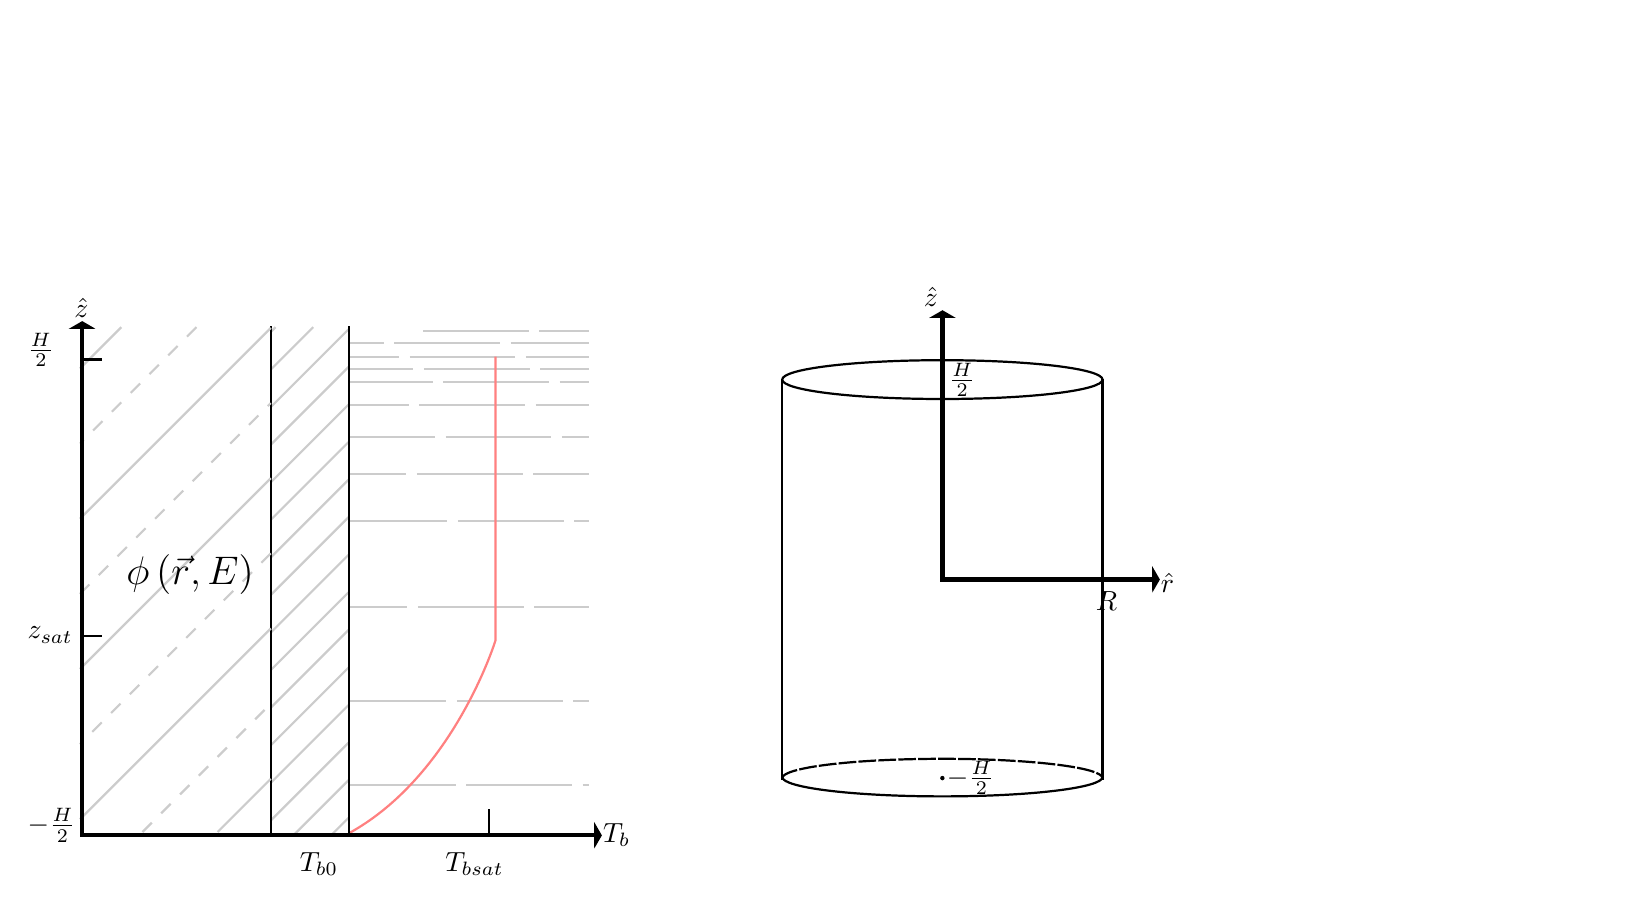
\begin{tikzpicture}[y=0.80pt, x=0.8pt,yscale=-1, inner sep=0pt, outer sep=0pt]
\begin{scope}[shift={(0,-782.35975)}]
    \path[shift={(0,782.35975)},rounded corners=0.0000cm] (110.6024,15.2892)
      rectangle (145.7349,244.3012);
    \path[shift={(0,782.35975)},draw=ccccccc,line width=0.800pt] (112.7854,15.2892)
      -- (110.6024,17.4722)(110.6024,34.4427) --
      (129.7560,15.2892)(145.7349,16.2807) -- (110.6024,51.4133)(110.6024,68.3838)
      -- (145.7349,33.2513)(145.7349,50.2219) --
      (110.6024,85.3544)(110.6024,102.3250) -- (145.7349,67.1924)(145.7349,84.1630)
      -- (110.6024,119.2955)(110.6024,136.2661) --
      (145.7349,101.1336)(145.7349,118.1041) --
      (110.6024,153.2367)(110.6024,170.2072) --
      (145.7349,135.0747)(145.7349,152.0453) --
      (110.6024,187.1778)(110.6024,204.1483) --
      (145.7349,169.0158)(145.7349,185.9864) --
      (110.6024,221.1189)(110.6024,238.0895) --
      (145.7349,202.9569)(145.7349,219.9275) --
      (121.3612,244.3012)(138.3318,244.3012) -- (145.7349,236.8981);
  \begin{scope}[shift={(0,782.35975)},fill=black]
  \end{scope}
  \path[fill=black] (260.69519,1032.1277) node[above right] (text5217) {$T_{b}$};
  \path[fill=black] (256.6422,1021.1097) -- (260.1554,1027.1948) --
    (256.7091,1033.1639) -- cycle;
  \path[draw=black,line join=miter,line cap=butt,line width=0.800pt]
    (110.8434,797.3236) -- (110.8434,1027.6368);
  \path[fill=black] (189.49055,1045.2996) node[above right] (text3075-4-9)
    {$T_{bsat}$};
  \path[shift={(0,782.35975)},draw=black,line join=miter,line cap=butt,line
    width=0.800pt] (209.3206,244.2375) -- (209.3206,232.7363);
    \path[shift={(0,782.35975)},rounded corners=0.0000cm] (24.3976,15.2892)
      rectangle (110.6024,243.3253);
    \path[shift={(0,782.35975)},draw=ccccccc,dash pattern=on 4.80pt off 4.80pt,miter
      limit=4.00,line width=0.800pt] (77.0174,15.2892) --
      (24.3976,67.9090)(24.3976,135.7912) -- (110.6024,49.5864)(110.6024,117.4686)
      -- (24.3976,203.6735)(52.6280,243.3253) -- (110.6024,185.3509);
  \begin{scope}[shift={(0,0)}]
      \path[shift={(0,782.35975)},rounded corners=0.0000cm] (24.3976,15.2892)
        rectangle (110.6024,243.3253);
      \path[shift={(0,782.35975)},draw=ccccccc,line width=0.800pt] (43.0763,15.2892)
        -- (24.3976,33.9678)(110.6024,15.6453) -- (24.3976,101.8501)(110.6024,83.5275)
        -- (24.3976,169.7323)(110.6024,151.4098) --
        (24.3976,237.6146)(110.6024,219.2920) -- (86.5691,243.3253);
  \end{scope}
  \path[draw=ccccccc,line join=miter,line cap=butt,line width=0.721pt]
    (179.3878,799.4232) -- (227.1421,799.4232);
  \path[draw=ccccccc,line join=miter,line cap=butt,line width=0.721pt]
    (231.9033,799.4232) -- (254.5107,799.4232);
  \path[draw=ccccccc,line join=miter,line cap=butt,line width=0.721pt]
    (145.9225,804.8659) -- (161.6221,804.8659);
  \path[draw=ccccccc,line join=miter,line cap=butt,line width=0.721pt]
    (166.3833,804.8659) -- (214.1376,804.8659);
  \path[draw=ccccccc,line join=miter,line cap=butt,line width=0.721pt]
    (218.8988,804.8659) -- (254.5028,804.8659);
  \path[draw=ccccccc,line join=miter,line cap=butt,line width=0.721pt]
    (145.9242,810.9134) -- (168.5863,810.9134);
  \path[draw=ccccccc,line join=miter,line cap=butt,line width=0.721pt]
    (173.3475,810.9134) -- (221.1017,810.9134);
  \path[draw=ccccccc,line join=miter,line cap=butt,line width=0.721pt]
    (225.8629,810.9134) -- (254.5045,810.9134);
  \path[draw=ccccccc,line join=miter,line cap=butt,line width=0.721pt]
    (145.9225,816.3561) -- (174.9819,816.3561);
  \path[draw=ccccccc,line join=miter,line cap=butt,line width=0.721pt]
    (179.7431,816.3561) -- (227.4974,816.3561);
  \path[draw=ccccccc,line join=miter,line cap=butt,line width=0.721pt]
    (232.2586,816.3561) -- (254.5038,816.3561);
  \path[draw=ccccccc,line join=miter,line cap=butt,line width=0.721pt]
    (145.9234,822.4035) -- (183.7937,822.4035);
  \path[draw=ccccccc,line join=miter,line cap=butt,line width=0.721pt]
    (188.5549,822.4035) -- (236.3092,822.4035);
  \path[draw=ccccccc,line join=miter,line cap=butt,line width=0.721pt]
    (241.0704,822.4035) -- (254.5038,822.4035);
  \path[draw=ccccccc,line join=miter,line cap=butt,line width=0.721pt]
    (145.9205,832.6842) -- (172.9922,832.6842);
  \path[draw=ccccccc,line join=miter,line cap=butt,line width=0.721pt]
    (177.7534,832.6842) -- (225.5076,832.6842);
  \path[draw=ccccccc,line join=miter,line cap=butt,line width=0.721pt]
    (230.2688,832.6842) -- (254.5078,832.6842);
  \path[draw=ccccccc,line join=miter,line cap=butt,line width=0.721pt]
    (145.9217,847.1981) -- (184.7886,847.1981);
  \path[draw=ccccccc,line join=miter,line cap=butt,line width=0.721pt]
    (189.5498,847.1981) -- (237.3040,847.1981);
  \path[draw=ccccccc,line join=miter,line cap=butt,line width=0.721pt]
    (242.0652,847.1981) -- (254.5057,847.1981);
  \path[draw=ccccccc,line join=miter,line cap=butt,line width=0.721pt]
    (145.9229,864.1310) -- (171.8552,864.1310);
  \path[draw=ccccccc,line join=miter,line cap=butt,line width=0.721pt]
    (176.6164,864.1310) -- (224.3706,864.1310);
  \path[draw=ccccccc,line join=miter,line cap=butt,line width=0.721pt]
    (229.1318,864.1310) -- (254.5106,864.1310);
  \path[draw=ccccccc,line join=miter,line cap=butt,line width=0.721pt]
    (145.9220,885.2971) -- (190.3315,885.2971);
  \path[draw=ccccccc,line join=miter,line cap=butt,line width=0.721pt]
    (195.0927,885.2971) -- (242.8469,885.2971);
  \path[draw=ccccccc,line join=miter,line cap=butt,line width=0.721pt]
    (247.6081,885.2971) -- (254.5043,885.2971);
  \path[draw=ccccccc,line join=miter,line cap=butt,line width=0.721pt]
    (145.9198,924.0009) -- (172.2815,924.0009);
  \path[draw=ccccccc,line join=miter,line cap=butt,line width=0.721pt]
    (177.0428,924.0009) -- (224.7970,924.0009);
  \path[draw=ccccccc,line join=miter,line cap=butt,line width=0.721pt]
    (229.5582,924.0009) -- (254.5073,924.0009);
  \path[draw=ccccccc,line join=miter,line cap=butt,line width=0.721pt]
    (145.9199,966.3331) -- (189.9051,966.3331);
  \path[draw=ccccccc,line join=miter,line cap=butt,line width=0.721pt]
    (194.6663,966.3331) -- (242.4206,966.3331);
  \path[draw=ccccccc,line join=miter,line cap=butt,line width=0.721pt]
    (247.1818,966.3331) -- (254.5013,966.3331);
  \path[draw=ccccccc,line join=miter,line cap=butt,line width=0.721pt]
    (146.4147,1004.4321) -- (194.1689,1004.4321);
  \path[draw=ccccccc,line join=miter,line cap=butt,line width=0.721pt]
    (198.9301,1004.4321) -- (246.6843,1004.4321);
  \path[draw=ccccccc,line join=miter,line cap=butt,line width=0.721pt]
    (251.4455,1004.4321) -- (254.5044,1004.4321);
  \path[fill=black] (19.3464,798.4296) -- (25.4315,794.9164) -- (31.4006,798.3627)
    -- cycle;
  \path[fill=black] (21.87632,793.11084) node[above right] (text5217-7)
    {$\hat{z}$};
  \path[fill=black] (123.6966,1045.2996) node[above right] (text3075-4-9-0)
    {$T_{b0}$};
  \path[shift={(0,782.35975)},draw=cff8080,line join=miter,line cap=butt,line
    width=0.800pt] (145.7349,243.9759) .. controls (193.2289,217.9518) and
    (212.0964,156.7952) .. (212.0964,156.7952) -- (212.0964,28.6265);
  \path[draw=black,line join=miter,line cap=butt,line width=0.800pt]
    (145.9759,797.3236) -- (145.9759,1027.6368);
  \path[fill=black] (45.397591,918.33563) node[above right] (text3113)
    {\Large{$\phi\left(\vec{r},E\right)$}};
  \path[draw=black,line join=miter,line cap=butt,line width=0.800pt]
    (24.7229,937.2031) -- (34.4819,937.2031);
  \path[fill=black] (0.79517746,940.34521) node[above right] (text3119)
    {$z_{sat}$};
  \path[draw=black,dash pattern=on 6.40pt off 1.60pt on 0.80pt off 1.60pt,line
    join=miter,line cap=butt,miter limit=4.00,line width=0.800pt]
    (24.7229,797.3236) -- (24.7229,1027.6368);
  \path[draw=black,line join=miter,line cap=butt,miter limit=4.00,line
    width=1.600pt] (258.4638,1027.1368) -- (25.2229,1027.1368) --
    (25.2229,797.3236);
  \path[fill=black] (0.79517746,1030.2789) node[above right] (text3119-4)
    {$-\frac{H}{2}$};
  \path[fill=black] (0.79517746,815.42957) node[above right] (text3119-4-8)
    {$\frac{H}{2}$};
  \path[draw=black,line join=miter,line cap=butt,line width=0.800pt]
    (24.7229,812.2875) -- (34.4819,812.2875);
  \path[shift={(0,782.35975)},draw=black,miter limit=4.00,line width=0.800pt]
    (486.2984,38.9710) .. controls (486.2984,43.8111) and (453.9070,47.7348) ..
    (413.9503,47.7348) .. controls (373.9935,47.7348) and (341.6022,43.8111) ..
    (341.6022,38.9710) .. controls (341.6022,34.1309) and (373.9935,30.2072) ..
    (413.9503,30.2072) .. controls (453.9070,30.2072) and (486.2984,34.1309) ..
    (486.2984,38.9710) -- cycle;
  \path[draw=black,line join=miter,line cap=butt,line width=0.800pt]
    (341.6022,821.1443) -- (341.6022,1002.0145);
  \path[draw=black,line join=miter,line cap=butt,line width=0.800pt]
    (486.2984,821.1443) -- (486.2984,1002.0145);
  \path[shift={(0,961.85285)},draw=black,miter limit=4.00,line width=0.800pt]
    (486.2984,38.9710) .. controls (486.2984,43.8111) and (453.9070,47.7348) ..
    (413.9503,47.7348) .. controls (373.9935,47.7348) and (341.6022,43.8111) ..
    (341.6022,38.9710) .. controls (341.6022,38.9710) and (341.6022,38.9710) ..
    (341.6022,38.9710);
  \path[cm={{-1.0,0.0,0.0,-1.0,(827.90058,1040.348)}},draw=black,dash pattern=on
    6.40pt off 0.80pt,miter limit=4.00,line width=0.800pt] (486.2984,38.9710) ..
    controls (486.2984,43.8111) and (453.9070,47.7348) .. (413.9503,47.7348) ..
    controls (373.9935,47.7348) and (341.6022,43.8111) .. (341.6022,38.9710) ..
    controls (341.6022,38.9710) and (341.6022,38.9710) .. (341.6022,38.9710);
  \path[draw=black,line join=miter,line cap=butt,miter limit=4.00,line
    width=1.600pt] (413.9503,791.8695) -- (413.9503,911.5794) --
    (510.9116,911.5794);
  \path[fill=black] (407.9232,793.5106) -- (414.0083,789.9974) --
    (419.9774,793.4437) -- cycle;
  \path[fill=black] (405.63022,788.19183) node[above right] (text5217-7-6)
    {$\hat{z}$};
  \path[fill=black] (508.6826,905.5523) -- (512.1958,911.6374) --
    (508.7496,917.6065) -- cycle;
  \path[fill=black] (512.60217,917.45496) node[above right] (text5217-7-6-2)
    {$\hat{r}$};
  \path[fill=black] (483.31491,925.80176) node[above right] (text4910) {$R$};
  \path[fill=black] (416.93369,829.00891) node[above right] (text4914)
    {$\frac{H}{2}$};
  \path[fill=black] (415.97266,1008.7836) node[above right] (text4914-2)
    {$-\frac{H}{2}$};
  \path[cm={{0.44691,0.0,0.0,0.44691,(276.78363,937.32384)}},fill=black]
    (309.1575,143.2044) .. controls (309.1575,144.4402) and (308.1557,145.4420) ..
    (306.9199,145.4420) .. controls (305.6841,145.4420) and (304.6823,144.4402) ..
    (304.6823,143.2044) .. controls (304.6823,141.9687) and (305.6841,140.9668) ..
    (306.9199,140.9668) .. controls (308.1557,140.9668) and (309.1575,141.9687) ..
    (309.1575,143.2044) -- cycle;
  \begin{scope}[shift={(607.12707,-135.27408)}]
    \path[shift={(0,782.35975)},rounded corners=0.0000cm] (24.3976,15.2892)
      rectangle (110.6024,243.3253);
  \end{scope}
  \begin{scope}[shift={(610.1105,-82.31828)}]
      \path[shift={(0,782.35975)},rounded corners=0.0000cm] (24.3976,15.2892)
        rectangle (110.6024,243.3253);
  \end{scope}
\end{scope}

\end{tikzpicture}
